\chapter{Activity V2}

\section{Sample Input File}

Alex Dickinson-Lomas from the University of Birmingham requested a calculation to predict the radioactivity of a thin 0.1mm piece of steel in a 5MeV proton beam.  A SRIM exyz file had been prepared and the following input file was set up.

\begin{lstlisting}[style=sOutputFile,caption={Activity V2 Input File}]
# Data files
data isotopes="/cloud/Code/python/activity/data/isotopes" xs="/cloud/Code/python/activity/data/xs"

# Sim
sim1 exyz="EXYZ.txt" target_composition=Fe,96.375,C,0.772,Cu,0.024,Mn,1.36,Ni,0.698,Si,0.381,Cr,0.092,V,0.008,P,0.009,Si,0.003,Mo,0.278 target_depth=0.1,mm target_density=7808,kgm3 beam_projectile='proton' beam_energy=5,MeV beam_area=64,mm2 beam_duration=300,s beam_current=0.5,uA end_time=260000,s
\end{lstlisting}




%%%%%%%%%%%%%%%%%%%%%%%%%%%%%%%%%%%%%%%%%%%%%%%%%%%%%%%%%%
\begin{comment}
\section{Sample Output}

The activity code processed the input file, and the calculation duration was approximately 15-20 minutes.

\lstinputlisting[style=sOutputFile,caption={Activity V2 Steel Terminal Output}]{appendix/activity_code/5mev/5mevsteel.txt}

\section{Output Plots}

The program produces many different plots, including those of the cross sections for each target isotope.  Four of the most important plots for the 5MeV proton irradiated steel are included here.

First is the total activity (fig. \ref{fig:activityv2-steel-5min-a}), from the time the beam starts until the beam is turned off.  It shows a steady rise in activity, and from this graph it is hard to see any curve towards a saturation of radioactive isotopes as the beam duration is so short.

\FloatBarrier

\begin{figure}
	\begin{center}
		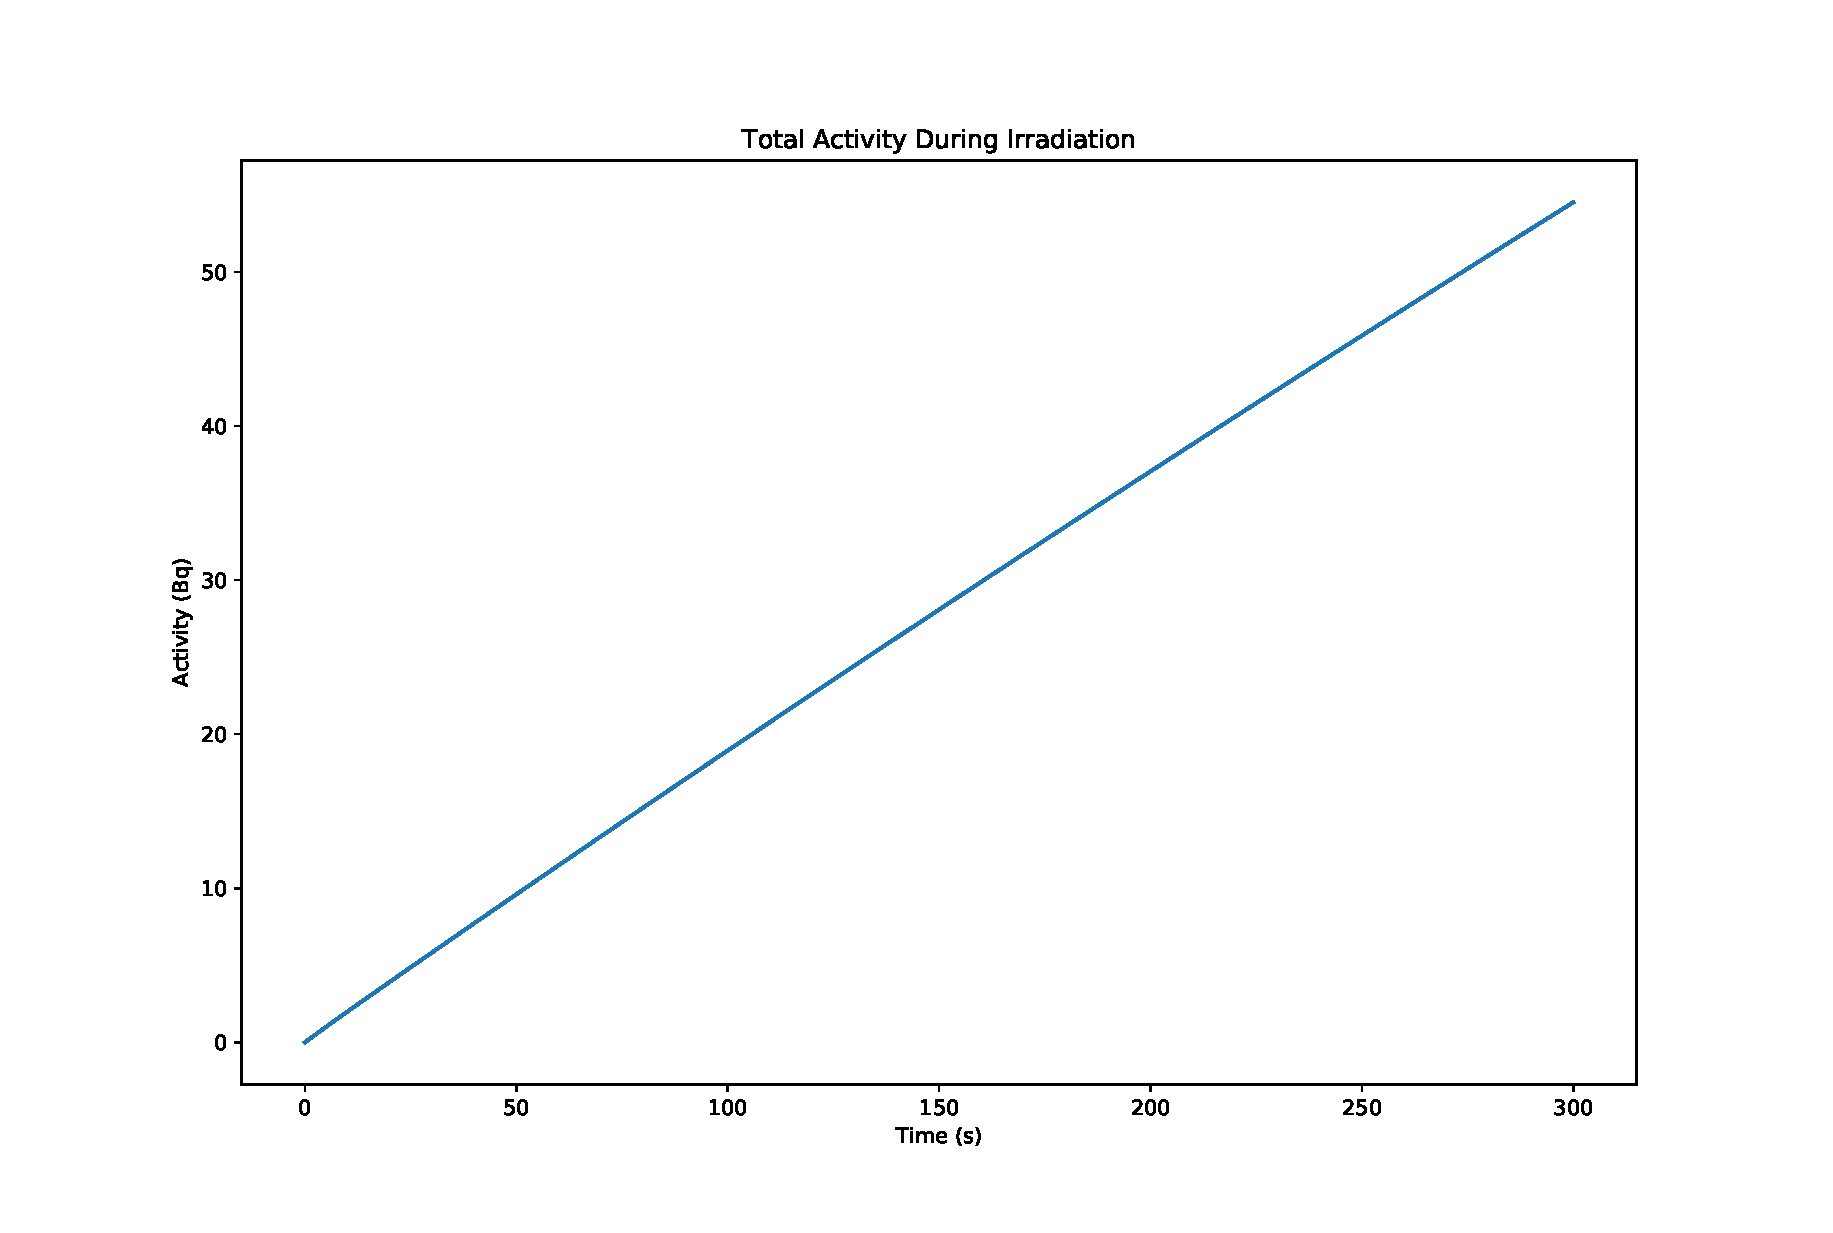
\includegraphics[width=0.8\linewidth]{appendix/activity_code/5mev/end_of_beam_000___total.eps}
		\captionsetup{font={it}}
		\caption{Total activity from all isotopes from the start to the end of the beam (during irradiation)}
		\label{fig:activityv2-steel-5min-a}
	\end{center}
\end{figure}
\FloatBarrier

The cooling period is much longer than the time spent within the beam, so a second graph shows the overall activity from when irradiation begins, to when it ceases up until the end of the simulation time (fig. \ref{fig:activityv2-steel-5min-b}).

\FloatBarrier

\begin{figure}
	\begin{center}
		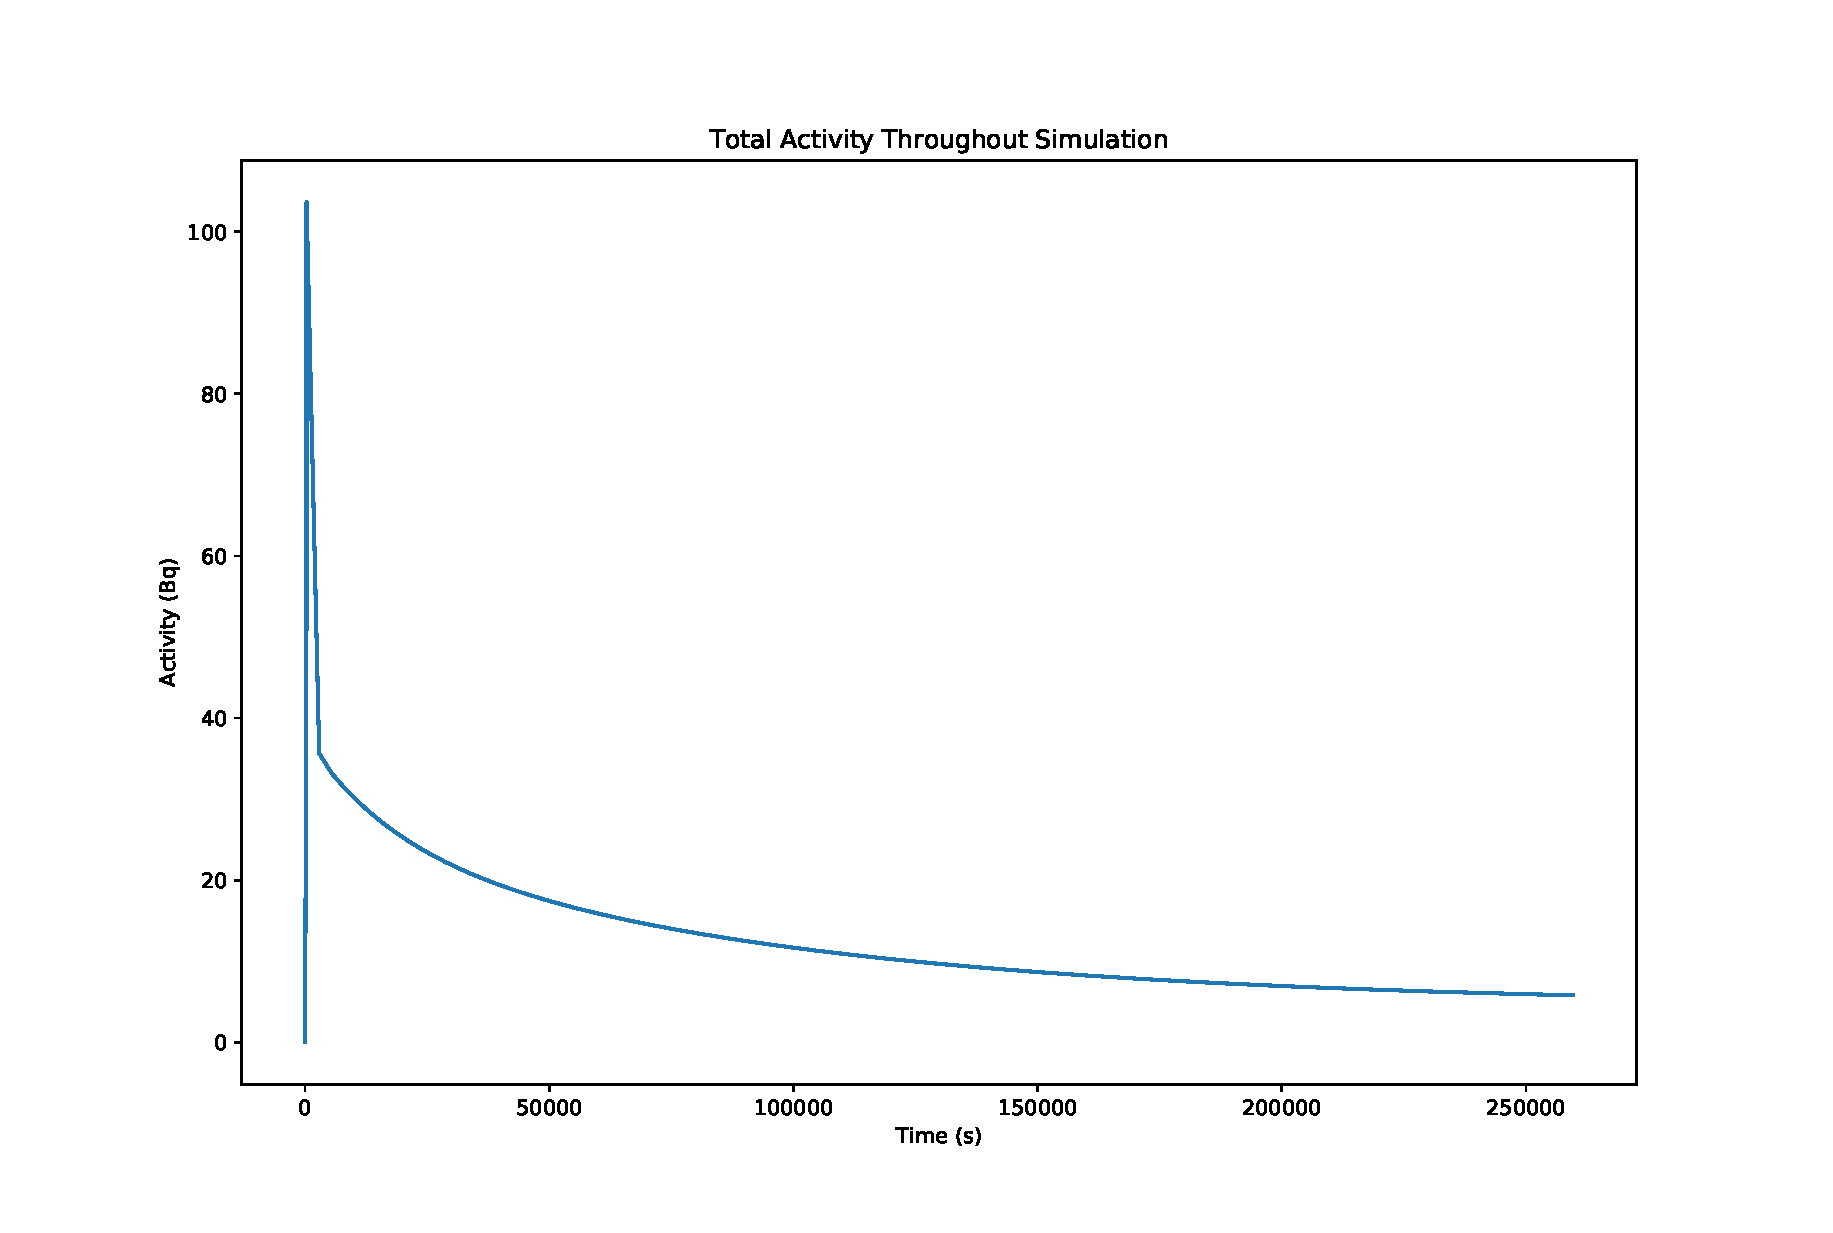
\includegraphics[width=0.8\linewidth]{appendix/activity_code/5mev/end_of_sim_000___total.eps}
		\captionsetup{font={it}}
		\caption{Total activity from all isotopes from the start to the end of the simulation}
		\label{fig:activityv2-steel-5min-b}
	\end{center}
\end{figure}
\FloatBarrier

The predicted gamma lines at the end of irradiation are predicted in the end of beam gamma line plot (fig. \ref{fig:activityv2-steel-5min-gammalines-a}).

\FloatBarrier

\begin{figure}
	\begin{center}
		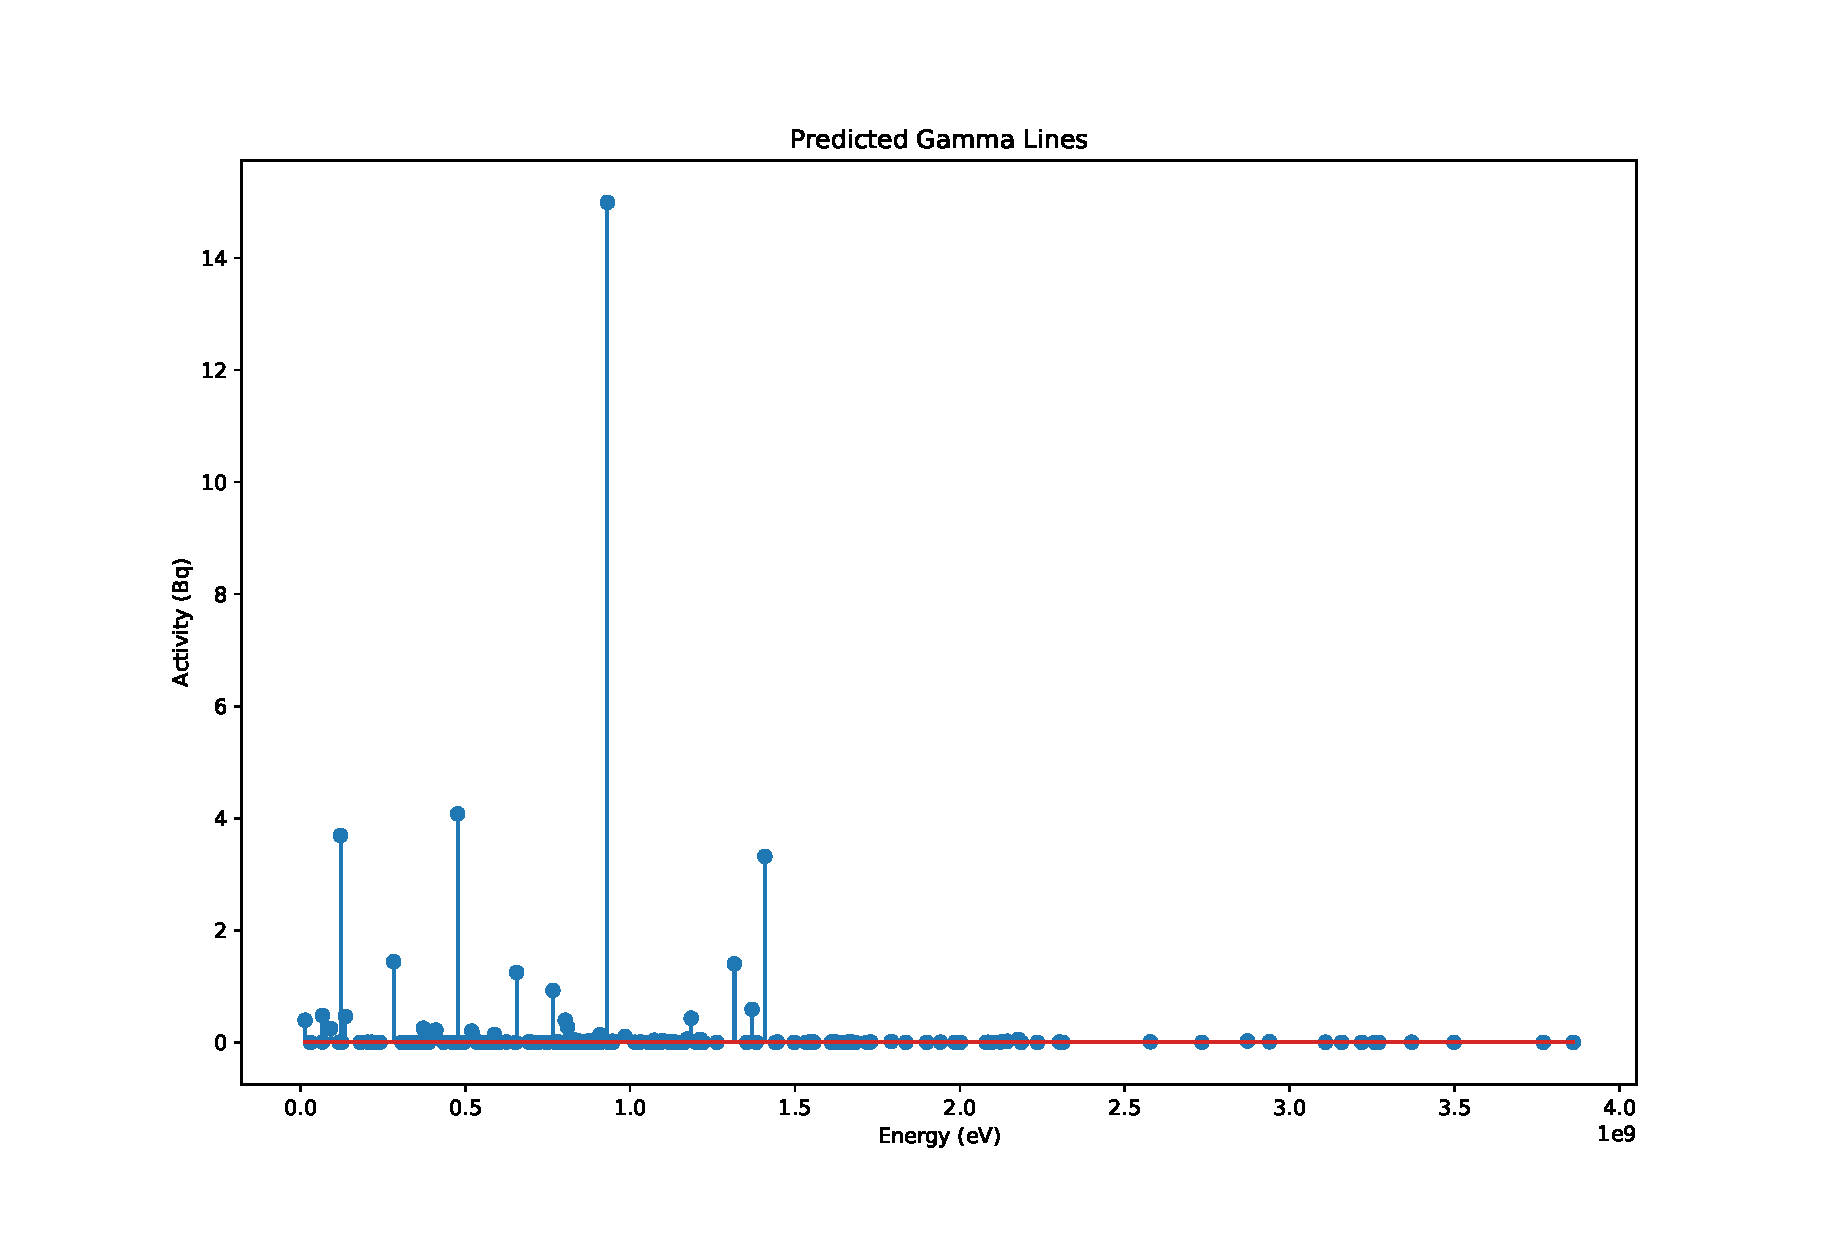
\includegraphics[width=0.8\linewidth]{appendix/activity_code/5mev/end_of_beam_gamma_lines.eps}
		\captionsetup{font={it}}
		\caption{Expected gamma lines and activity at the end of irradiation}
		\label{fig:activityv2-steel-5min-gammalines-a}
	\end{center}
\end{figure}
\FloatBarrier

The predicted gamma lines at the end of simulation are predicted in the end of sim gamma line plot (fig. \ref{fig:activityv2-steel-5min-gammalines-b}).

\FloatBarrier

\begin{figure}
	\begin{center}
		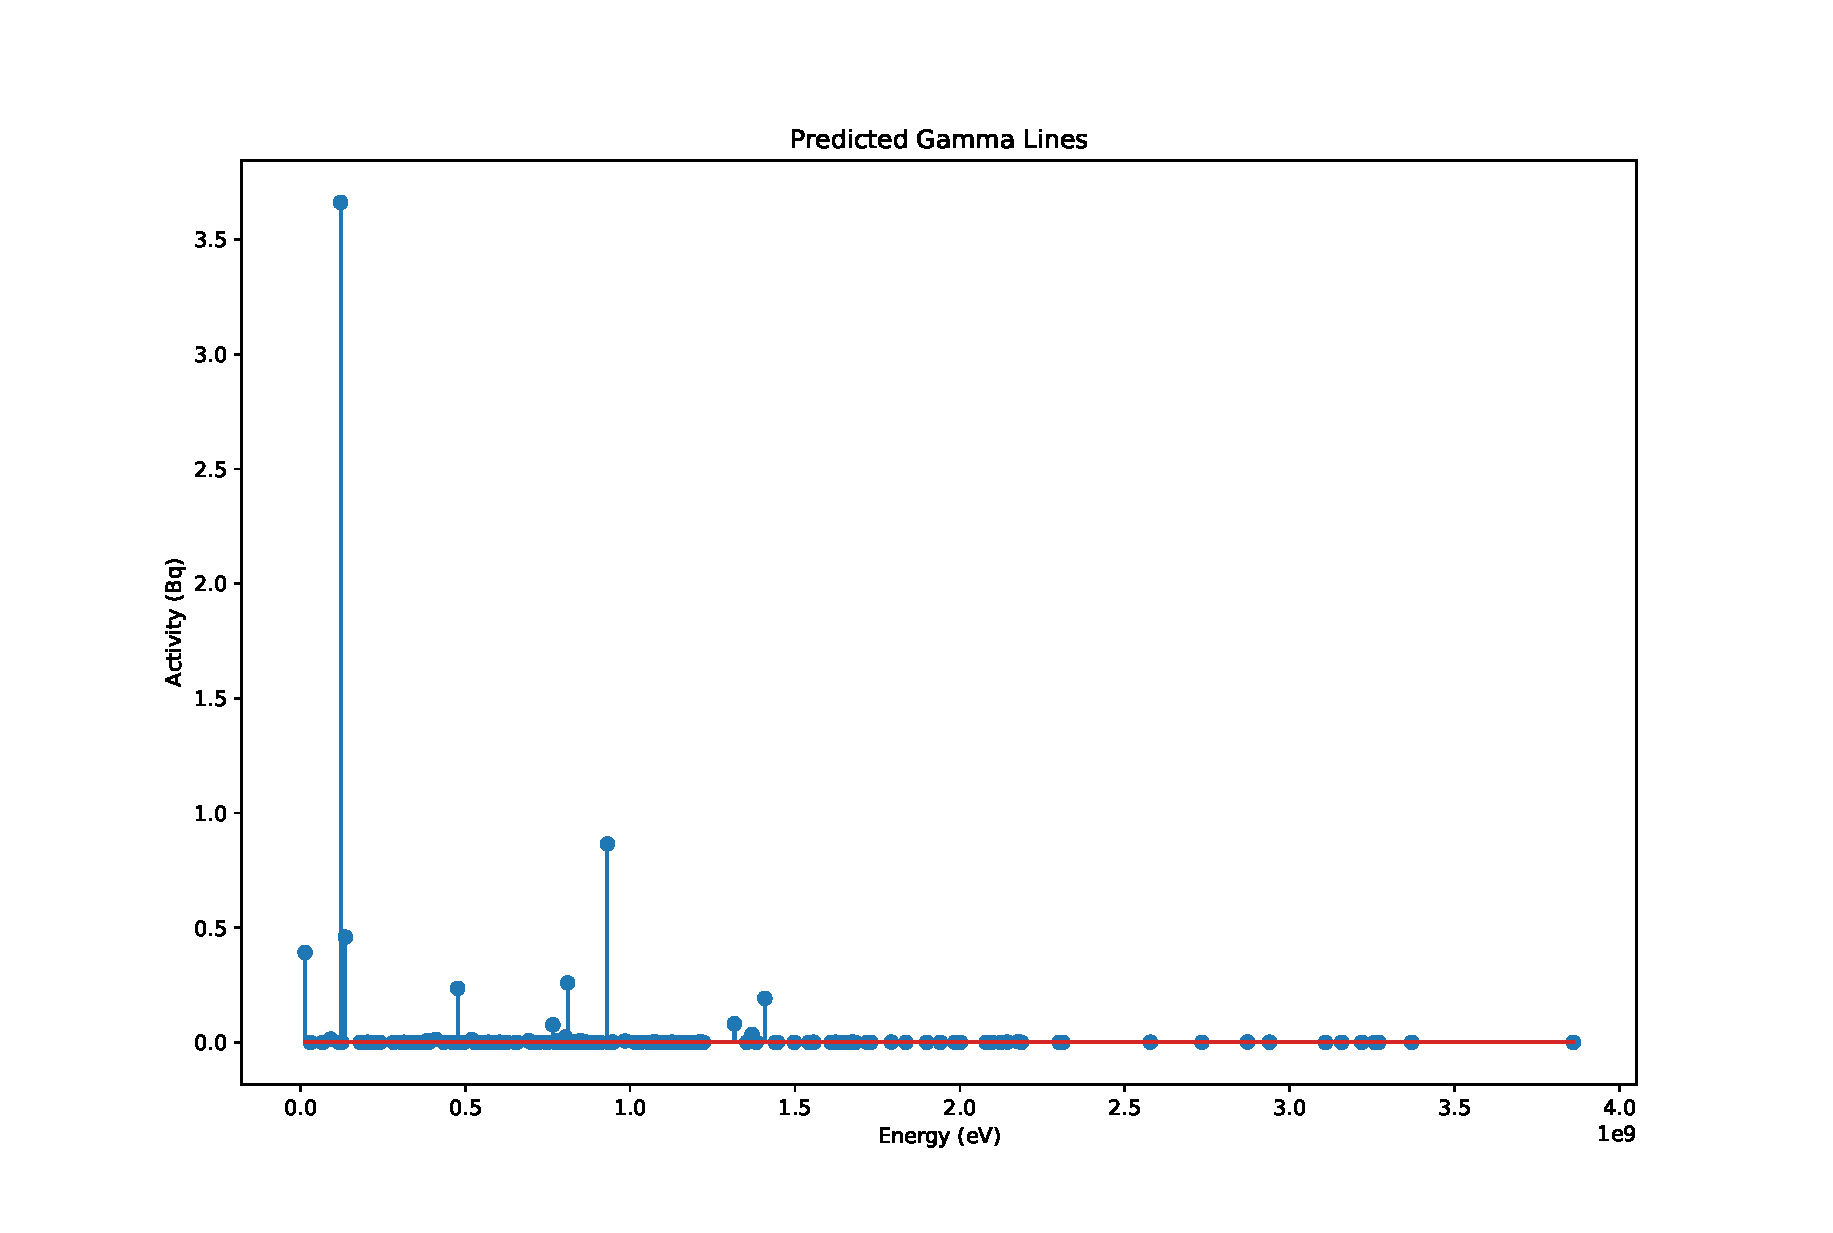
\includegraphics[width=0.8\linewidth]{appendix/activity_code/5mev/end_of_sim_gamma_lines.eps}
		\captionsetup{font={it}}
		\caption{Expected gamma lines and activity at the end of the simulation}
		\label{fig:activityv2-steel-5min-gammalines-b}
	\end{center}
\end{figure}
\FloatBarrier

\FloatBarrier
\section{An Example to Show Saturation In Beam}

With the first steel example, the beam duration was too short to show a saturation of radioactive isotopes.  This shows the gradual levelling off of activity during irradiation over a day as the source rate begins to equalize with the decay rate \
(fig. \ref{fig:activityv2-steel-1day}).

\begin{lstlisting}[style=sOutputFile,caption={Activity V2 input file: steel irradiated for 1 day}]
# Data files
data isotopes="/cloud/Code/python/activity/data/isotopes" xs="/cloud/Code/python/activity/data/xs"

# Sim
sim1 exyz="EXYZ.txt" target_composition=Fe,96.375,C,0.772,Cu,0.024,Mn,1.36,Ni,0.698,Si,0.381,Cr,0.092,V,0.008,P,0.009,Si,0.003,Mo,0.278 target_depth=0.1,mm target_density=7808,kgm3 beam_projectile='proton' beam_energy=5,MeV beam_area=64,mm2 beam_duration=86400,s beam_current=0.5,uA end_time=864000,s
\end{lstlisting}


\begin{figure}
	\begin{center}
		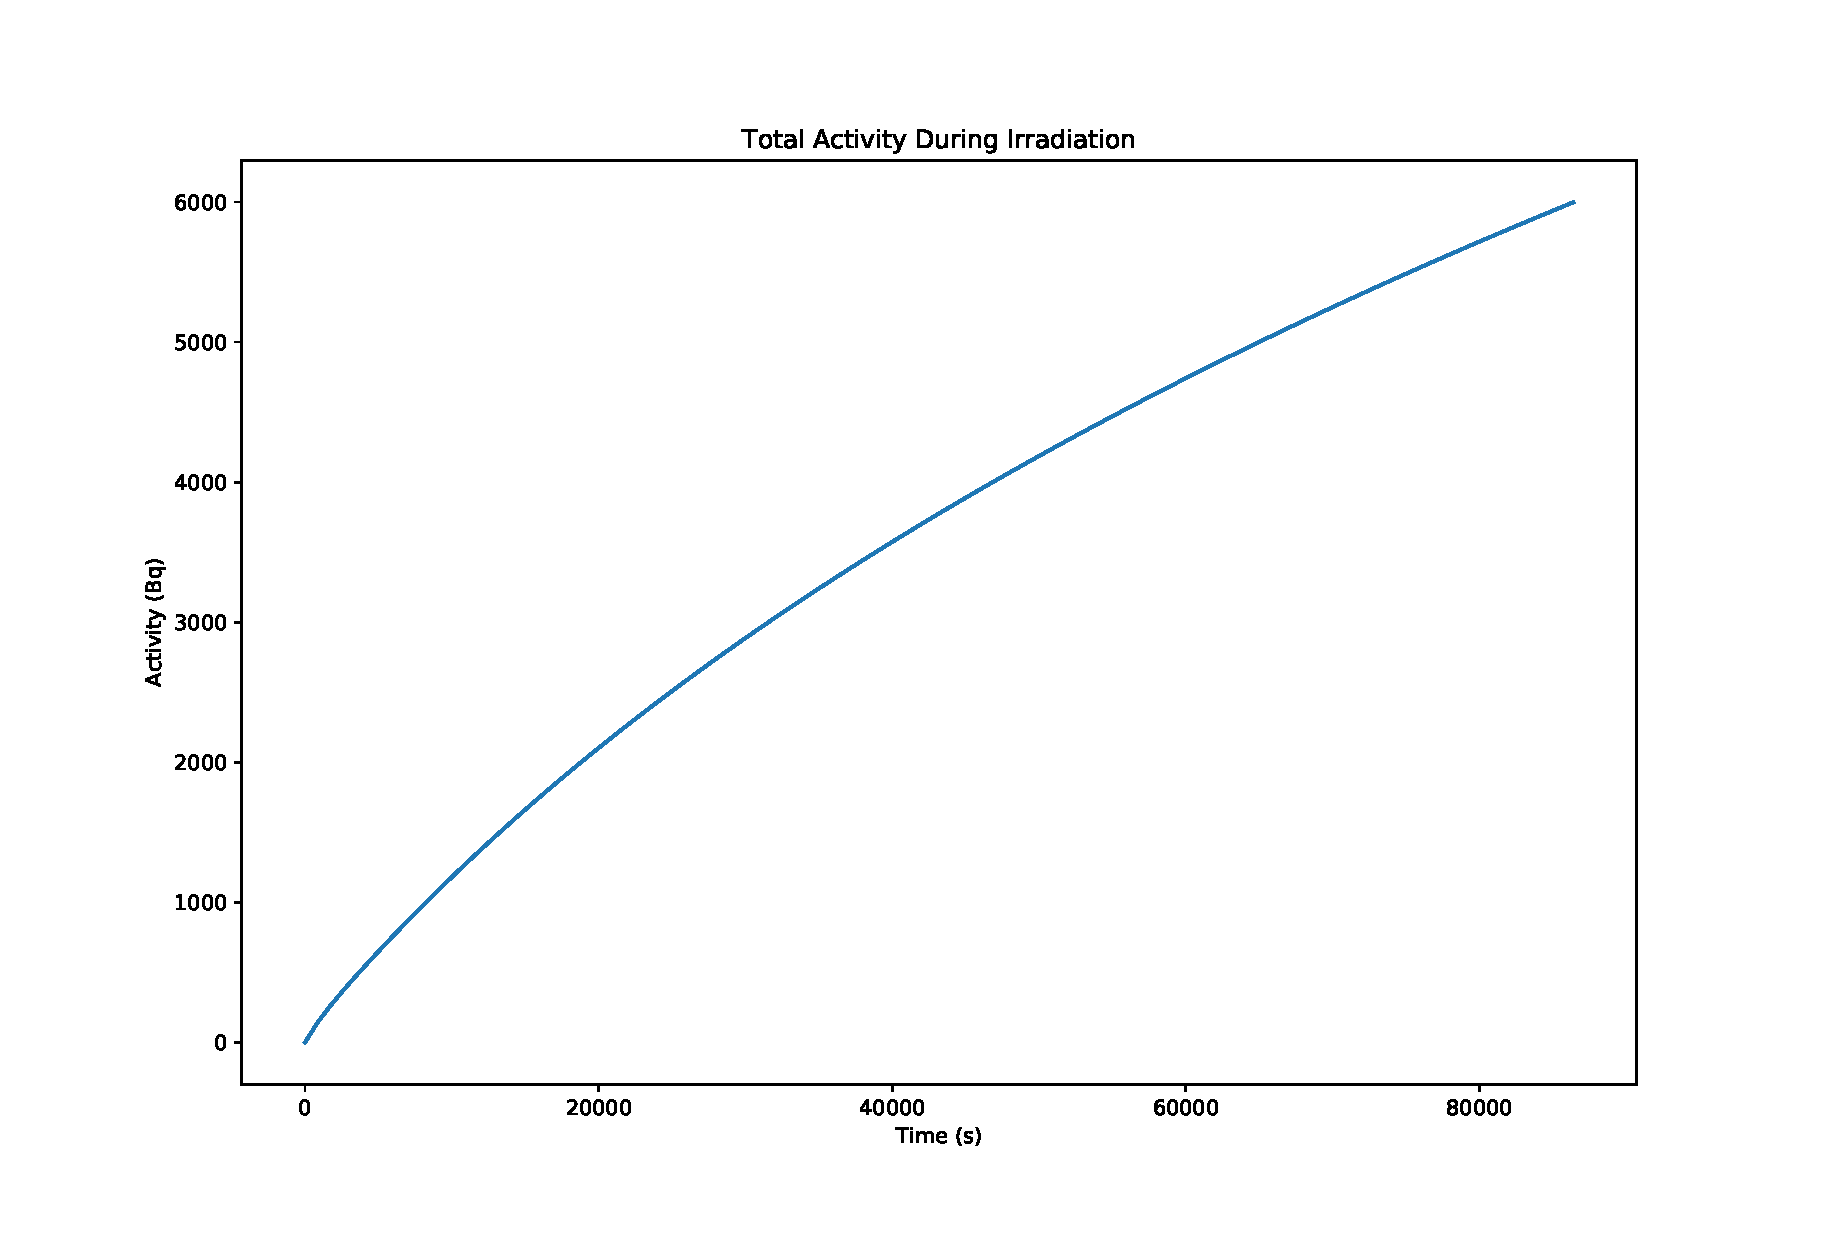
\includegraphics[width=0.8\linewidth]{appendix/activity_code/5mev_long/total.eps}
		\captionsetup{font={it}}
		\caption{Gradual saturation of steel with radioactive isotopes under proton irradiation}
		\label{fig:activityv2-steel-1day}
	\end{center}
\end{figure}
\FloatBarrier
\end{comment}
%%%%%%%%%%%%%%%%%%%%%%%%%%%%%%%%%%%%%%%%%%%%%%%%%%%%%%%%%%




\FloatBarrier
\section{Accompanying Manual}
\label{section:activityv2manual}



\includepdf[
    clip=0mm 0mm 0mm 0mm,
    trim=0mm 0mm 0mm 0mm,
    pages=-,
    frame,
    scale=.90,
    pagecommand={}]{appendix/activity_code/activity_v2_manual.pdf}


